\documentclass[conference]{IEEEtran}
% Based on the IEEE Conference Template (conference_101719.tex) on Overleaf.
\usepackage{cite}
\usepackage{amsmath,amssymb,amsfonts}
\usepackage{algorithmic}
\usepackage{graphicx}
\usepackage{textcomp}
\usepackage{xcolor}
\usepackage{array}
\usepackage{adjustbox}
\graphicspath{{figures/}}
\def\BibTeX{{\rm B\kern-.05em{\sc i\kern-.025em b}\kern-.08em
    T\kern-.1667em\lower.7ex\hbox{E}\kern-.125emX}}
\newcommand{\Qs}{Q^{*}}
\newcommand{\eps}{\varepsilon}
\begin{document}

\title{Learning the Pickup and Delivery Order of a Multi-Parcel Robot with Tabular Q-Learning, SARSA and Monte Carlo ES}

\author{\IEEEauthorblockN{Nguyen Quang Trung}
\IEEEauthorblockA{\textit{Student ID: 22011211} \\
\textit{Phenikaa University}\\
Hanoi, Vietnam}
}

\maketitle

\begin{abstract}
A robot on a grid must pick up several parcels and deliver each one to its own drop cell, choosing the order by itself. We model the task as a deterministic Markov decision process with four maps of increasing difficulty: more parcels, a capacity of one, a delivery deadline, and a booster cell that doubles the capacity for one trip. A deadline clock and a booster flag are added to the state to keep it Markov, which brings the largest map to 357,696 encoded states (15,612 reachable). We compare three tabular methods, Q-learning, SARSA and Monte Carlo with exploring starts (MC ES), trained with exploring starts, algorithm-specific exploration schedules and a numba-compiled training loop that is about 150--180 times faster than a Python loop. Accuracy is measured as the share of start cells from which the greedy policy reaches the optimal return computed by value iteration. All three methods reach 100\% accuracy on all four maps in 5/5 seeds, against 0--61\% with the original settings on the two hardest maps. Q-learning learns fastest, MC ES is second and SARSA needs about three times as many episodes. Changing the late penalty, the deadline or the booster cell changes the learned delivery order exactly as the optimal solution predicts.
\end{abstract}

\begin{IEEEkeywords}
reinforcement learning, Q-learning, SARSA, Monte Carlo exploring starts, pickup and delivery, tabular methods
\end{IEEEkeywords}

\section{Introduction}
In a pickup and delivery problem, a vehicle collects goods at given locations and brings each item to its own destination \cite{b9}. The order of visits decides the route length, and constraints such as a vehicle capacity or a delivery deadline make some orders infeasible or costly. Instead of solving the routing problem directly, this work lets an agent learn the order from rewards alone.

The environment extends the Taxi domain \cite{b4}, \cite{b5} from one passenger to several parcels, and adds a capacity limit, a deadline and a booster cell. Because the environment is small and deterministic, value iteration gives the exact optimal policy, which makes it possible to measure how close each learned policy is to the optimum, not only whether it reaches the goal.

The contributions are:
\begin{itemize}
\item a \texttt{gymnasium} environment \cite{b5} with four maps of increasing difficulty, each adding one mechanic, and a Markov state that includes a deadline clock and a booster flag;
\item a comparison of Q-learning \cite{b2}, SARSA \cite{b3} and MC ES \cite{b1} under the same exploring-starts protocol, with exploration schedules chosen per algorithm;
\item a strict accuracy measure over every start cell, and an ablation showing that exploring starts and the new schedules raise accuracy from as low as 0\% to 100\%;
\item experiments that change the reward and the environment, and value heatmaps that show how the deadline and the booster appear in the learned values.
\end{itemize}

\section{Environment and MDP Formulation}

\subsection{Rules and Rewards}
The robot moves on an $H\times W$ grid with walls. Each parcel $i$ has a pickup cell and a drop cell. There are six actions: Up, Down, Left and Right move one cell (a move into a wall or off the grid leaves the robot in place), Pickup takes a waiting parcel in the current cell if the capacity allows it, and Drop delivers a carried parcel in its drop cell. Every step costs $-1$, a delivery earns $+20$, a wrong Pickup or Drop costs an extra $-10$, and a deadline parcel that is still undelivered when its deadline expires costs $-30$ once. An episode terminates when every parcel is delivered and is truncated after \texttt{max\_steps} steps (100, 150, 200 and 300 on the four maps).

\subsection{State and Markov Property}
A state is the tuple
\begin{equation}
s=(r,\,c,\,\sigma_1,\dots,\sigma_N,\,\tau,\,b),\label{eq:state}
\end{equation}
where $(r,c)$ is the robot cell, $\sigma_i\in\{0,1,2\}$ means that parcel $i$ is waiting, carried or delivered, $\tau\in\{0,\dots,T_d\}$ counts the steps toward the deadline $T_d$, and $b\in\{0,1,2\}$ means that the booster is unused, active or used up. Without $\tau$, two visits to the same cell with the same parcel statuses could have different futures, and without $b$ the result of Pickup would depend on the history; both are therefore part of the state. Once the deadline parcel is delivered, $\tau$ is set to $T_d$ because time no longer affects the reward, which merges states that would otherwise be duplicated.

\subsection{Encoding and State-Space Size}
The parcel statuses are read as a base-3 number, and the tuple is packed into one integer that indexes the Q table:
\begin{align}
\mathrm{code}&=\textstyle\sum_{i=1}^{N}\sigma_i\,3^{\,i-1},\\
\mathrm{idx}&=\big(((rW+c)\,3^{N}+\mathrm{code})\,T+\tau\big)B+b,\label{eq:idx}
\end{align}
with $T=T_d+1$ on maps with a deadline ($T=1$ otherwise) and $B=3$ on the map with a booster ($B=1$ otherwise). The encoded size is $|S|=H\,W\,3^{N}\,T\,B$. Far fewer states are reachable (Table~\ref{tab:levels}): walls cannot be occupied, a capacity of one excludes two carried parcels, and $\tau$ and $b$ only take values that can actually occur. The reachable set is found by breadth-first search.

\subsection{Four Levels}
Each map adds one mechanic to the previous one (Fig.~\ref{fig:maps}, Table~\ref{tab:levels}). S1 has two parcels that can be carried together. S2 has three parcels and a capacity of one, so the order matters. S3 requires parcel C to be delivered within 20 steps. S4 has four parcels, a 22-step deadline for parcel D and a booster cell that allows two parcels to be carried for one trip; the trip ends the first time the robot is empty-handed after a Drop. S3 and S4 contain trade-offs: on S3 the route $B\rightarrow A\rightarrow C$ would be 4 steps shorter without the deadline, and on S4 the robot must deliver D first and then detour through the booster cell to carry A and B together, which saves 8 steps.

\begin{figure*}[!t]
\centering
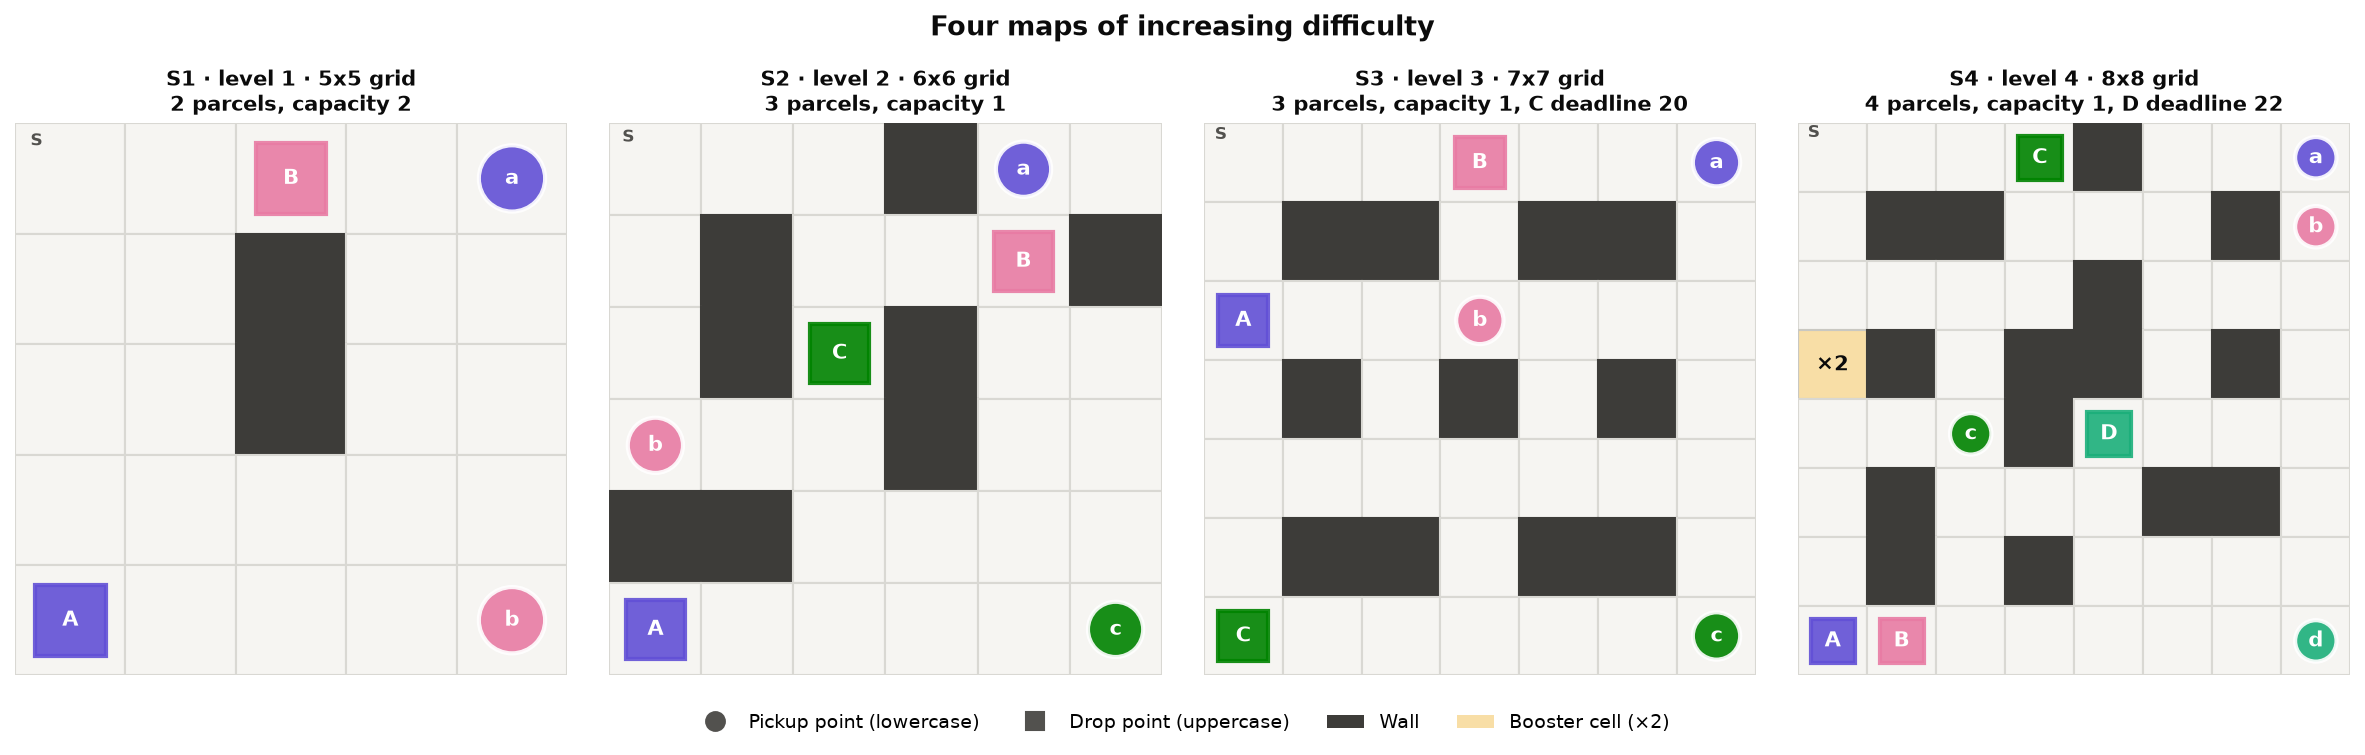
\includegraphics[width=\textwidth]{maps.png}
\caption{The four maps by level. Pickup cells are circles (lowercase letters), drop cells are squares (uppercase letters), walls are dark and the $\times 2$ booster cell is yellow.}
\label{fig:maps}
\end{figure*}

\begin{table*}[!t]
\caption{The Four Levels, Their State-Space Size and Optimal Routes (Value Iteration)}
\label{tab:levels}
\centering
\footnotesize
\begin{adjustbox}{max width=\textwidth}
\begin{tabular}{|c|c|c|c|p{4.6cm}|r|r|c|c|}
\hline
\textbf{Map} & \textbf{Grid} & \textbf{Parcels} & \textbf{Capacity} & \textbf{New mechanic} & \textbf{Encoded $|S|$} & \textbf{Reachable} & \textbf{Optimal route (steps, return)} & \textbf{max\_steps} \\
\hline
S1 & $5\times5$ & 2 & 2 & two parcels carried together & 225 & 186 & $A\rightarrow B$ (22, 18) & 100 \\
S2 & $6\times6$ & 3 & 1 & one parcel at a time, order matters & 972 & 535 & $B\rightarrow A\rightarrow C$ (36, 24) & 150 \\
S3 & $7\times7$ & 3 & 1 & parcel C within 20 steps & 27,783 & 4,027 & $C\rightarrow B\rightarrow A$ (44, 16) & 200 \\
S4 & $8\times8$ & 4 & 1 (2 with booster) & booster cell and parcel D within 22 steps & 357,696 & 15,612 & $D\rightarrow C\rightarrow B\rightarrow A$ (67, 13) & 300 \\
\hline
\end{tabular}
\end{adjustbox}
\end{table*}

\section{Learning Algorithms}
All three methods keep a table $Q(s,a)$ of size $|S|\times 6$ and act greedily with respect to it after training, $\pi(s)=\arg\max_a Q(s,a)$. They differ only in the target used to update $Q$.

\subsection{Exploring Starts and Exploration Schedules}
Every training episode starts in a reachable state drawn uniformly at random (any parcel statuses, $\tau$ and $b$), and its first action is also random. Every pair $(s,a)$ is therefore updated directly, including states such as ``carrying C at $\tau=15$'' that a robot starting at $\tau=0$ rarely visits. Evaluation still starts with every parcel waiting. After the first action, Q-learning and SARSA act $\eps$-greedily with an exponentially decaying $\eps$,
\begin{equation}
\eps(ep)=\eps_{s}\left(\frac{\eps_{e}}{\eps_{s}}\right)^{\min\left(1,\;ep/(f\,n_{ep})\right)},
\end{equation}
where $n_{ep}$ is the number of episodes and $f$ the fraction of training over which $\eps$ decays (Table~\ref{tab:hyper}).

\subsection{Q-Learning}
Q-learning \cite{b2} updates after every step toward
\begin{equation}
y=\begin{cases} r, & \text{if } s' \text{ is terminal},\\ r+\gamma\max_{a'}Q(s',a'), & \text{otherwise},\end{cases}\label{eq:ql}
\end{equation}
with $Q(s,a)\leftarrow Q(s,a)+\alpha\,[y-Q(s,a)]$. A truncated episode is not terminal, so the bootstrap term is kept on its last step. Because the target uses the best next action, Q-learning learns $\Qs$ while it explores (off-policy). The environment is deterministic, so the target has no noise and $\alpha=1$ is used.

\subsection{SARSA}
SARSA \cite{b3} replaces the maximum by the action $a'$ that the $\eps$-greedy policy actually takes in $s'$:
\begin{equation}
y=r+\gamma\,Q(s',a').\label{eq:sarsa}
\end{equation}
It learns the value of the policy it is running (on-policy) and converges to $\Qs$ only when exploration vanishes in the limit (GLIE) \cite{b7}. The target is noisy through $a'$, so $\alpha$ decays linearly from 0.5 to 0.1, and $\eps$ decays to $10^{-5}$ during the first half of training.

\subsection{Monte Carlo with Exploring Starts}
MC ES \cite{b1} runs the greedy policy ($\eps=0$) after the random first pair, computes the returns backwards,
\begin{equation}
G_t=r_{t+1}+\gamma\,G_{t+1},
\end{equation}
and updates the first visit of each pair, $Q(s,a)\leftarrow Q(s,a)+\alpha\,[G_t-Q(s,a)]$. All exploration comes from the random start. With a greedy policy in a deterministic environment, the return after $(s,a)$ is a fixed number for the current policy, so $\alpha=1$ is used instead of the sample average $1/N$, which would keep the very negative returns of early, looping policies for a long time. A looping policy is cut at \texttt{max\_steps} with a very negative return, so the action that caused the loop is penalised on the next visit.

\subsection{Optimal Reference and Accuracy}
Value iteration \cite{b8} over all reachable states,
\begin{equation}
V(s)\leftarrow\max_a\big[r(s,a)+\gamma\,V(s')\big],
\end{equation}
gives the optimal return and $\Qs$. It is used only as a reference. The \emph{accuracy} of a policy is the share of start cells $c$ (every empty cell, every parcel waiting) from which the greedy policy obtains exactly the optimal return $R^{*}(c)$:
\begin{equation}
\mathrm{Acc}=\frac{1}{|C|}\sum_{c\in C}\mathbf{1}\big[R^{\pi}(c)=R^{*}(c)\big].
\end{equation}
This is stricter than checking the single start cell S, as Section~\ref{sec:ablation} shows.

\subsection{Implementation}
Since the environment is deterministic, the transition function is precomputed once into three arrays: next state $NS[s,a]$, reward $R[s,a]$ and termination flag $D[s,a]$. The training loops only look up these arrays and are compiled with numba \cite{b6}. On S2 with 20,000 episodes, one Q-learning run drops from 10.7~s to 0.06~s and one MC run from 15.4~s to 0.10~s, a speed-up of about 150--180 times. Table~\ref{tab:hyper} lists the final settings, which were tuned on the same four maps with 5 seeds.

\begin{table}[!t]
\caption{Hyperparameters (New Settings)}
\label{tab:hyper}
\centering
\footnotesize
\begin{adjustbox}{max width=\columnwidth}
\begin{tabular}{|l|c|c|c|}
\hline
 & \textbf{Q-learning} & \textbf{SARSA} & \textbf{MC ES} \\
\hline
$\gamma$ & \multicolumn{3}{c|}{0.99} \\
$\alpha$ & 1 & $0.5\rightarrow0.1$ (linear) & 1 \\
$\eps$ & $1\rightarrow0.01$ & $1\rightarrow10^{-5}$ & 0 \\
$\eps$ decay, $f$ & exponential, 0.8 & exponential, 0.5 & -- \\
Start state & \multicolumn{3}{c|}{exploring starts (random state and first action)} \\
$Q_0$ & \multicolumn{3}{c|}{0} \\
Episodes & \multicolumn{3}{c|}{S1: 100k, S2: 300k, S3: 2M, S4: 6M} \\
Seeds & \multicolumn{3}{c|}{5 per algorithm and map} \\
Evaluation & \multicolumn{3}{c|}{200 times per run (greedy, $\eps=0$)} \\
\hline
\end{tabular}
\end{adjustbox}
\end{table}

\section{Experiments and Results}

\subsection{Setup}
Each algorithm is trained on each map with 5 seeds. Every run is evaluated 200 times; each evaluation runs the greedy policy from cell S (return and success) and from every start cell (accuracy). The old settings, used for the ablation, start from a random empty cell with $\tau=0$ and $b=0$, decay $\eps$ linearly from 1 to 0.05 over 70\% of training, use $\alpha=0.5$, and average MC returns with $1/N$; they are run with the same number of episodes.

\subsection{Accuracy}
All 60 runs (3 algorithms $\times$ 4 maps $\times$ 5 seeds) end with 100\% accuracy and the optimal return from S, delivering on time on S3 and S4 (Fig.~\ref{fig:accuracy}). The learned Q tables also converge to $\Qs$: the final mean error $|Q-\Qs|$ is 0 for Q-learning and MC ES and between 0.001 and 0.047 for SARSA. Table~\ref{tab:first} shows when each method first reaches 100\%. Q-learning is the fastest on three maps; MC ES is slightly faster on S3 (median 290k against 350k episodes) because its greedy training episodes are short. On S4 the medians are 1.14M episodes for Q-learning, 1.74M for MC ES and 3.57M for SARSA. One seed on S4 (6M episodes) takes 38~s with Q-learning, 23~s with SARSA and 38~s with MC ES, and the full set of experiments takes 221~s on a 12-core CPU.

\begin{figure*}[!t]
\centering
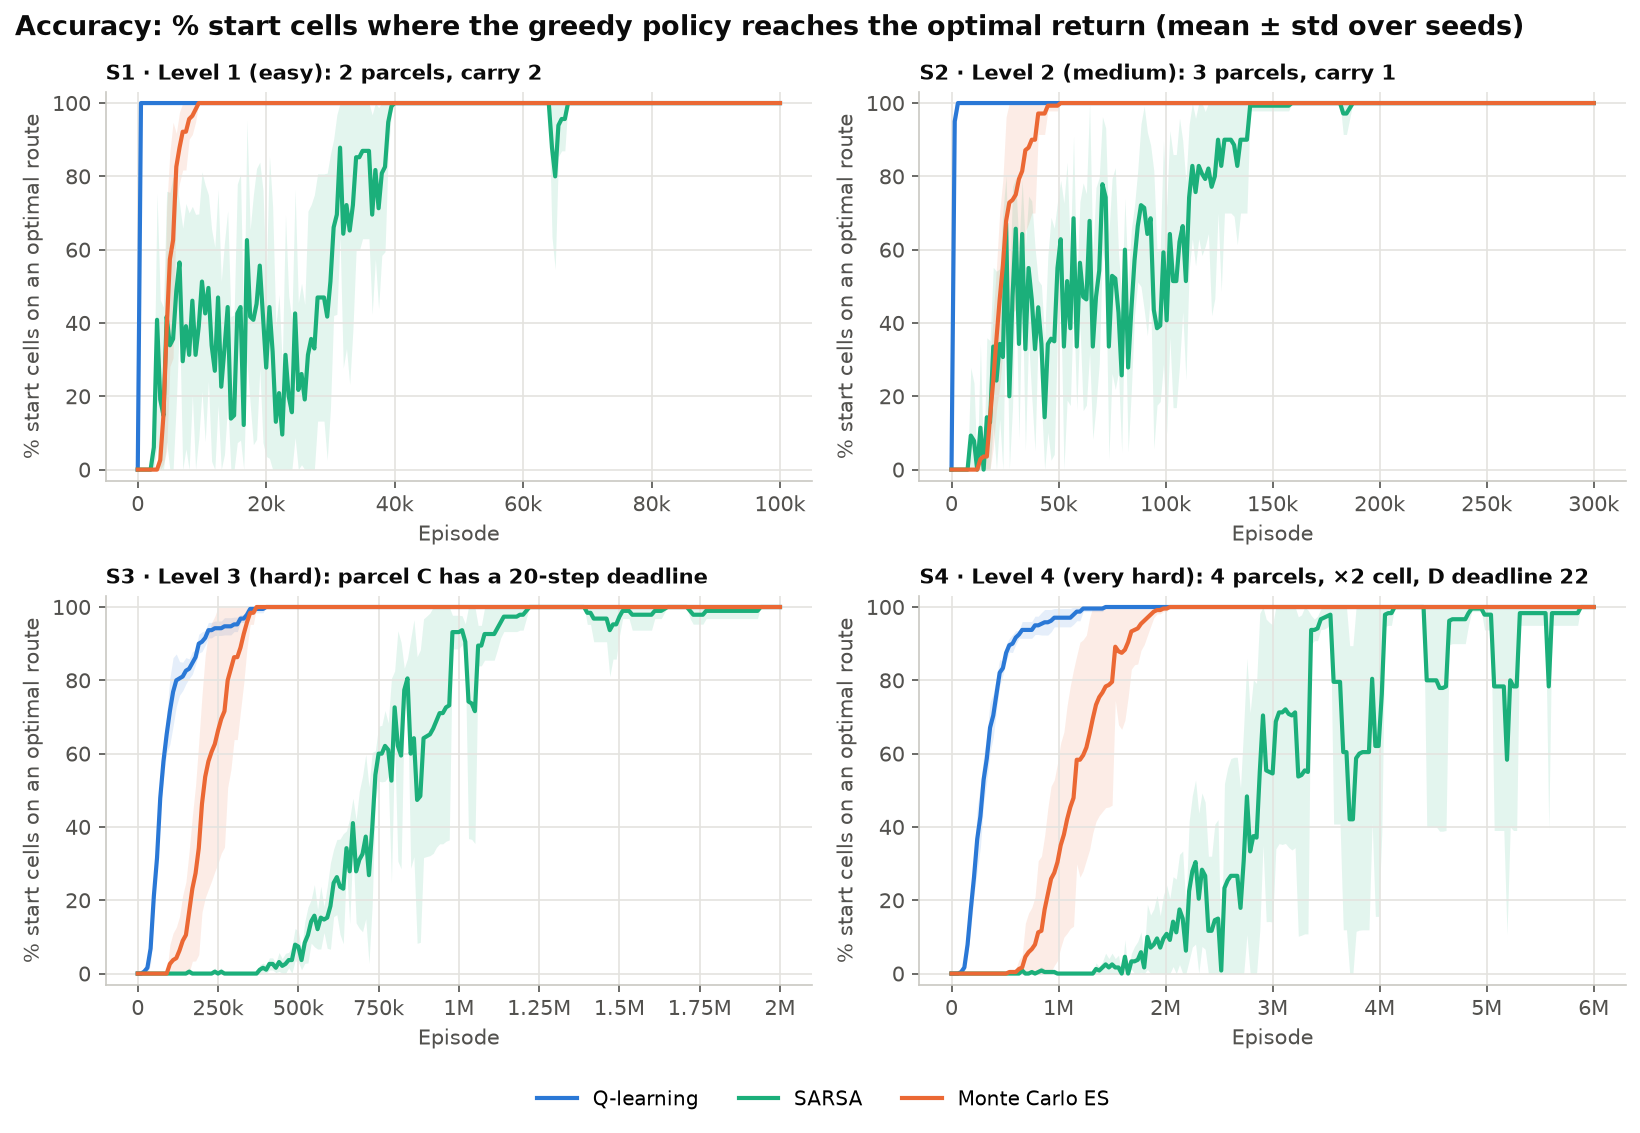
\includegraphics[width=0.82\textwidth]{accuracy.png}
\caption{Accuracy over training episodes: share of start cells from which the greedy policy reaches the optimal return, mean $\pm$ standard deviation over 5 seeds.}
\label{fig:accuracy}
\end{figure*}

\begin{table}[!t]
\caption{Episode at Which Accuracy First Reaches 100\% (Range over 5 Seeds)}
\label{tab:first}
\centering
\footnotesize
\begin{adjustbox}{max width=\columnwidth}
\begin{tabular}{|c|c|c|c|}
\hline
\textbf{Map (opt.)} & \textbf{Q-learning} & \textbf{SARSA} & \textbf{MC ES} \\
\hline
S1 (18) & 0.5k & 5.5k--33.5k & 7.0k--9.5k \\
S2 (24) & 1.5k--3.0k & 64.5k--159k & 30k--51k \\
S3 (16) & 340k--400k & 980k--1.22M & 260k--370k \\
S4 (13) & 840k--1.44M & 3.45M--4.14M & 1.47M--2.04M \\
\hline
\end{tabular}
\end{adjustbox}
\end{table}

\subsection{Effect of the Improvements}\label{sec:ablation}
With the same number of episodes, the old settings fail on the harder maps (Fig.~\ref{fig:ablation}, Table~\ref{tab:ablation}). On S3 and S4, SARSA and MC either deliver late (returns of $-18$ to $-30$ on S3) or do not finish before \texttt{max\_steps} (returns of $-290$ to $-330$ in 3/5 SARSA seeds and 4/5 MC seeds on S4). The old Q-learning follows the optimal route from S in all 5 seeds on S3 and S4, but it is correct from only 20\% and 61\% of the start cells: it memorised one route rather than solving the task, which a check from S alone would not reveal. The decisive change is exploring starts. The $\tau$ and $b$ dimensions multiply the number of states, and states away from the usual route are almost never updated when every episode starts at $\tau=0$. A final $\eps$ of 0.05 also biases SARSA toward the value of a policy that acts randomly 5\% of the time.

\begin{figure*}[!t]
\centering
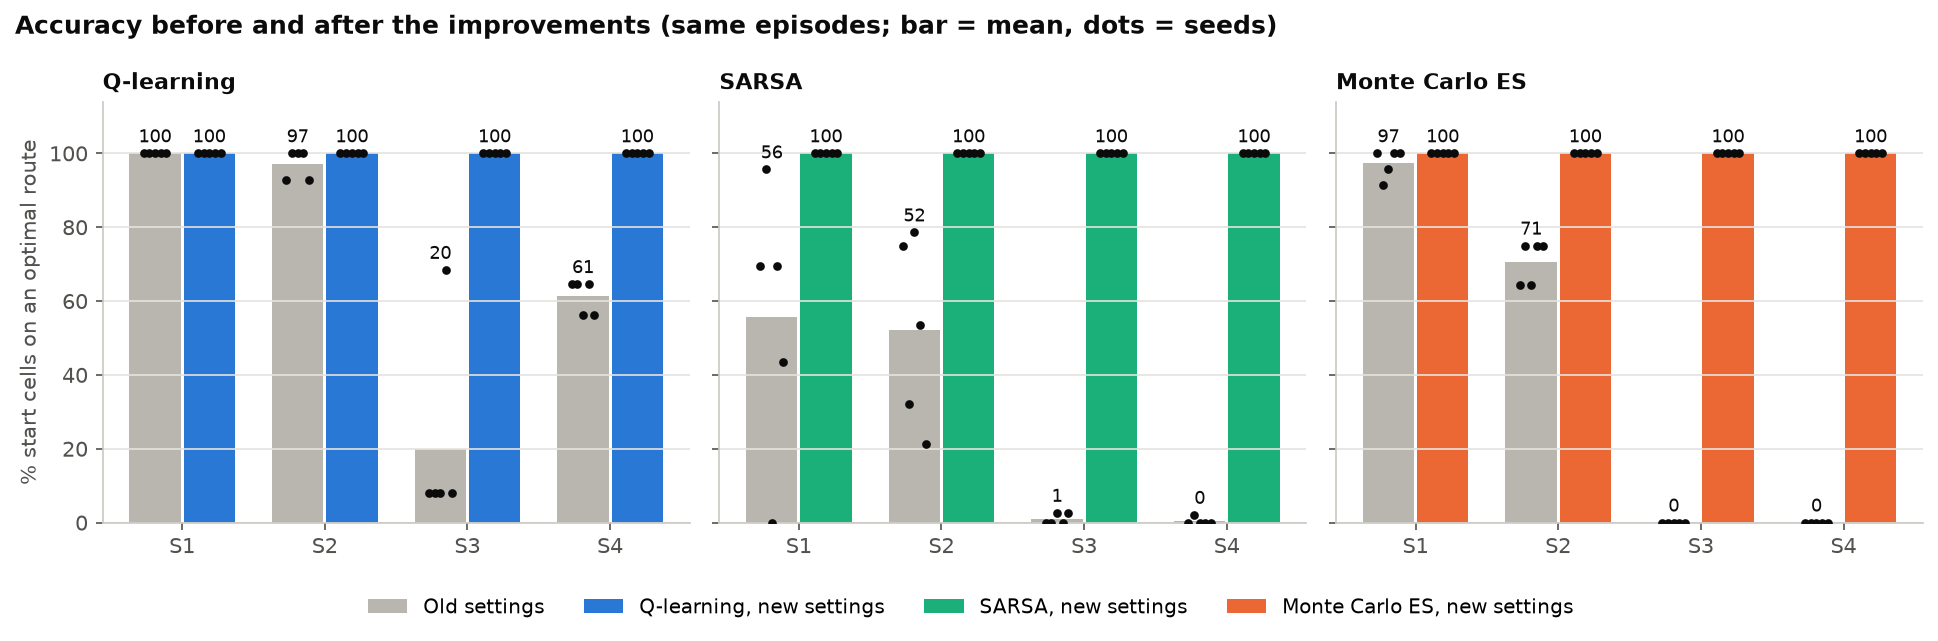
\includegraphics[width=\textwidth]{ablation.png}
\caption{Final accuracy with the old settings (grey) and the new settings (colour), with the same number of episodes. Bars show the mean, dots the individual seeds.}
\label{fig:ablation}
\end{figure*}

\begin{table}[!t]
\caption{Final Accuracy: Old Settings $\rightarrow$ New Settings}
\label{tab:ablation}
\centering
\footnotesize
\begin{adjustbox}{max width=\columnwidth}
\begin{tabular}{|c|c|c|c|}
\hline
\textbf{Map} & \textbf{Q-learning} & \textbf{SARSA} & \textbf{MC} \\
\hline
S1 & 100\% $\rightarrow$ 100\% & 55.7\% $\rightarrow$ 100\% & 97.4\% $\rightarrow$ 100\% \\
S2 & 97.1\% $\rightarrow$ 100\% & 52.1\% $\rightarrow$ 100\% & 70.7\% $\rightarrow$ 100\% \\
S3 & 20.0\% $\rightarrow$ 100\% & 1.1\% $\rightarrow$ 100\% & 0\% $\rightarrow$ 100\% \\
S4 & 61.3\% $\rightarrow$ 100\% & 0.4\% $\rightarrow$ 100\% & 0\% $\rightarrow$ 100\% \\
\hline
\end{tabular}
\end{adjustbox}
\end{table}

\subsection{Comparison of the Three Algorithms}
Since all three methods reach the optimum, they are compared on speed, stability and sensitivity to settings (Table~\ref{tab:compare}). \emph{Q-learning} is the fastest and the most stable: it learns $\Qs$ from every step, including random exploratory steps, and its target is noise-free, so $\alpha=1$ gives the exact value at once. It is also the least sensitive to the settings, still reaching 100\% on S1 and 97\% on S2 with the old ones. \emph{MC ES} is second. It updates only at the end of an episode, which slows the early phase, but greedy returns in a deterministic environment are exact, so it converges to $\Qs$ like Q-learning. It depends entirely on exploring starts and reaches 0\% on S3 and S4 without them. \emph{SARSA} is the slowest, needing about three times as many episodes as Q-learning on S4. It learns the value of its exploring policy and matches $\Qs$ only once $\eps$ is very small, and its noisy target makes actions with nearly equal values swap, so its accuracy still dips after first reaching 100\%. Per second, however, a SARSA episode is the cheapest. Its usual advantage, safer behaviour while exploring, does not appear here because the maps contain no dangerous cells.

\begin{table*}[!t]
\caption{Comparison of the Three Algorithms (Medians over 5 Seeds Where Applicable)}
\label{tab:compare}
\centering
\footnotesize
\begin{adjustbox}{max width=\textwidth}
\begin{tabular}{|l|c|c|c|}
\hline
\textbf{Criterion} & \textbf{Q-learning} & \textbf{SARSA} & \textbf{MC ES} \\
\hline
Update & after every step & after every step & after the episode \\
Target & $r+\gamma\max Q(s')$, no noise & $r+\gamma Q(s',a')$, noisy through $a'$ & return $G$, no noise with $\eps=0$ \\
Learns the value of & the optimal policy (off-policy) & its $\eps$-greedy policy (on-policy) & its greedy policy (on-policy) \\
Episodes to 100\% on S4 & 1.14M & 3.57M & 1.74M \\
Mean accuracy during training (S1/S2/S3/S4) & 0.99 / 0.99 / 0.95 / 0.94 & 0.77 / 0.77 / 0.60 / 0.48 & 0.95 / 0.91 / 0.89 / 0.80 \\
Drops below 100\% after reaching it & never & 9--19\% of evaluations & never \\
Final mean error $|Q-\Qs|$ & 0 & 0.001--0.047 & 0 \\
Time per seed on S4 & 38 s & 23 s & 38 s \\
Old settings, final accuracy (S1/S2/S3/S4) & 100 / 97 / 20 / 61\% & 56 / 52 / 1 / 0.4\% & 97 / 71 / 0 / 0\% \\
\hline
\end{tabular}
\end{adjustbox}
\end{table*}

\subsection{Learned Policy and Value Function}
On S4 the learned policy matches the optimal solution (Fig.~\ref{fig:policy}): the robot picks up D in the bottom-right corner and delivers it in the middle of the map before its deadline, delivers C on the top row, goes down to the $\times2$ cell to switch the booster on, picks up A and B in the top-right corner, and delivers both in the bottom-left corner, finishing in 67 steps with return 13. The agent has learned both trade-offs: it prioritises the deadline parcel although it is far away, and it accepts a detour to use the booster.

Fig.~\ref{fig:value_start} colours every cell by the learned value $V(s)=\max_a Q(s,a)$ for a start with every parcel waiting. The value at S is 13.7, 17.8, 8.6 and 2.5 on S1--S4, below the undiscounted optimal returns (18, 24, 16, 13) because later rewards are discounted by $\gamma=0.99$. Fig.~\ref{fig:value_phases} shows the value in four phases of the S4 route. Within a phase, cells near the current target are darker, so the greedy robot walks toward darker cells. The deadline appears as a cliff: in phase 2 (carrying D, $\tau=15$) the cells far from D's drop cell fall to about $-11$, because from there D cannot arrive in time and the $-30$ penalty is certain. In phase 8 the robot carries A and B together, and almost the whole map is dark because two $+20$ rewards are a few steps away.

\begin{figure*}[!t]
\centering
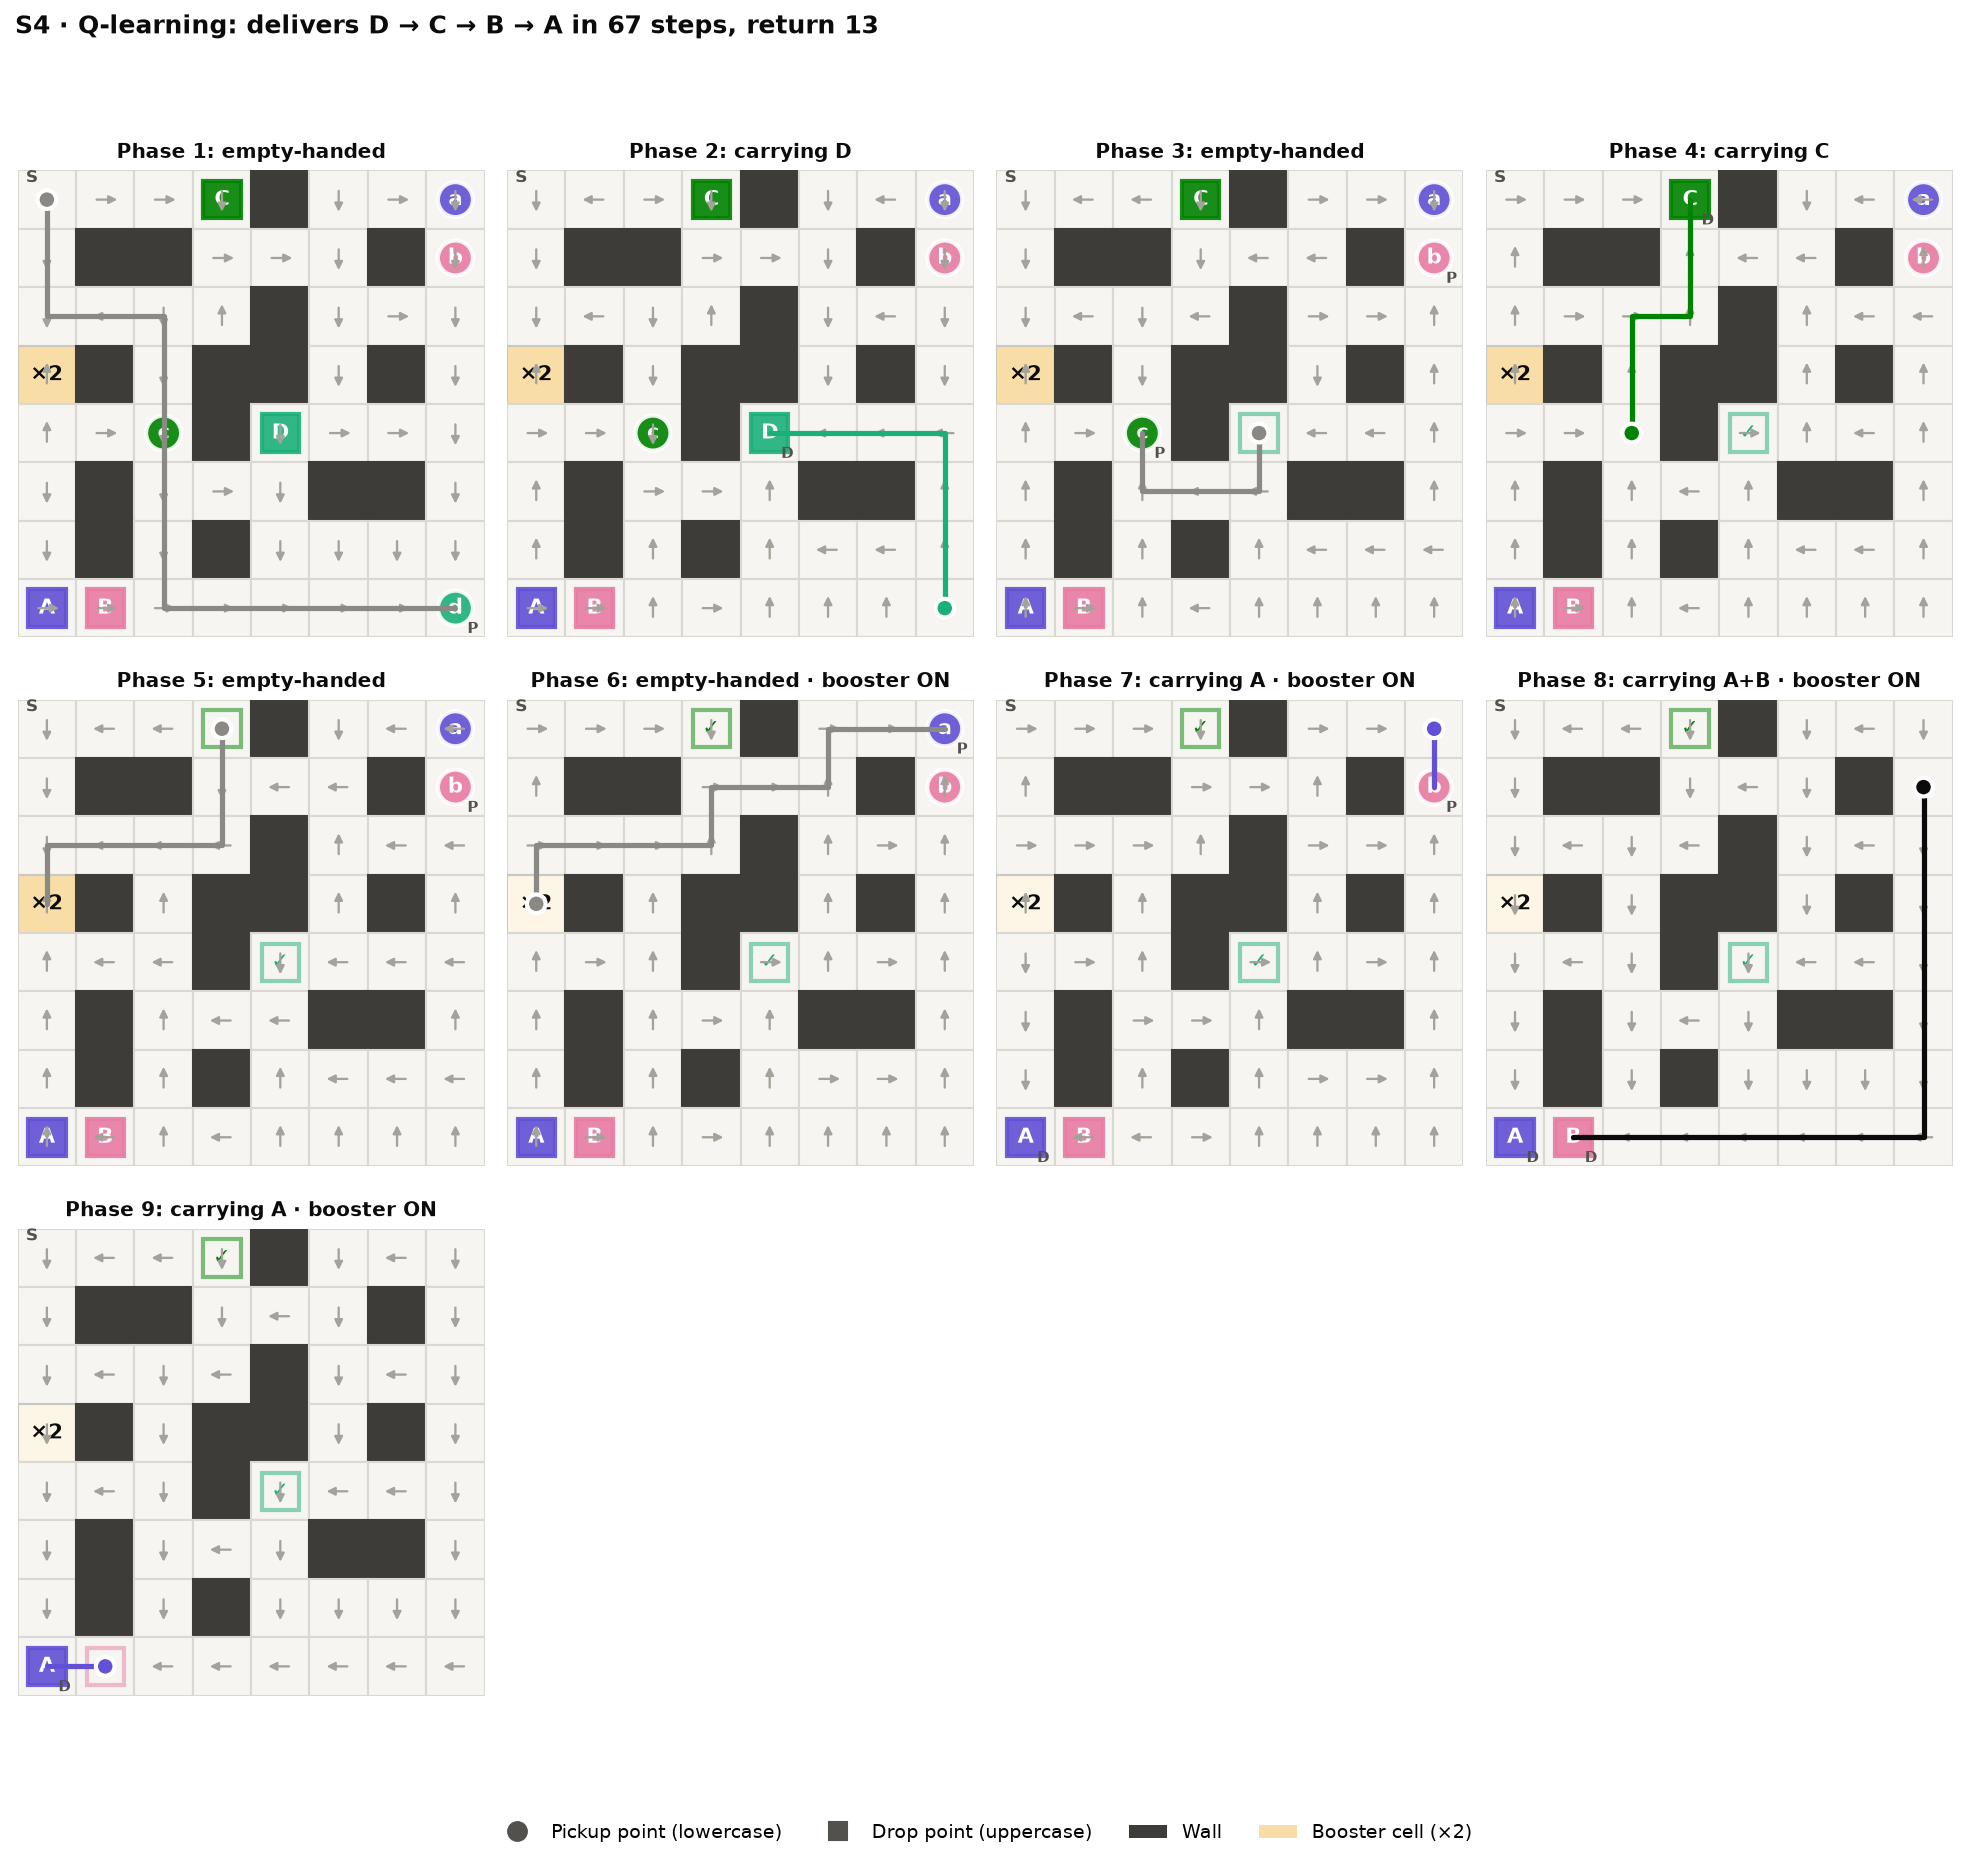
\includegraphics[width=0.62\textwidth]{policy_S4.png}
\caption{S4 policy learned by Q-learning, one panel per phase (parcel and booster status). Grey arrows: greedy action in each cell; P/D: Pickup/Drop. The coloured line is the actual route, coloured by the parcel carried (black: two parcels).}
\label{fig:policy}
\end{figure*}

\begin{figure*}[!t]
\centering
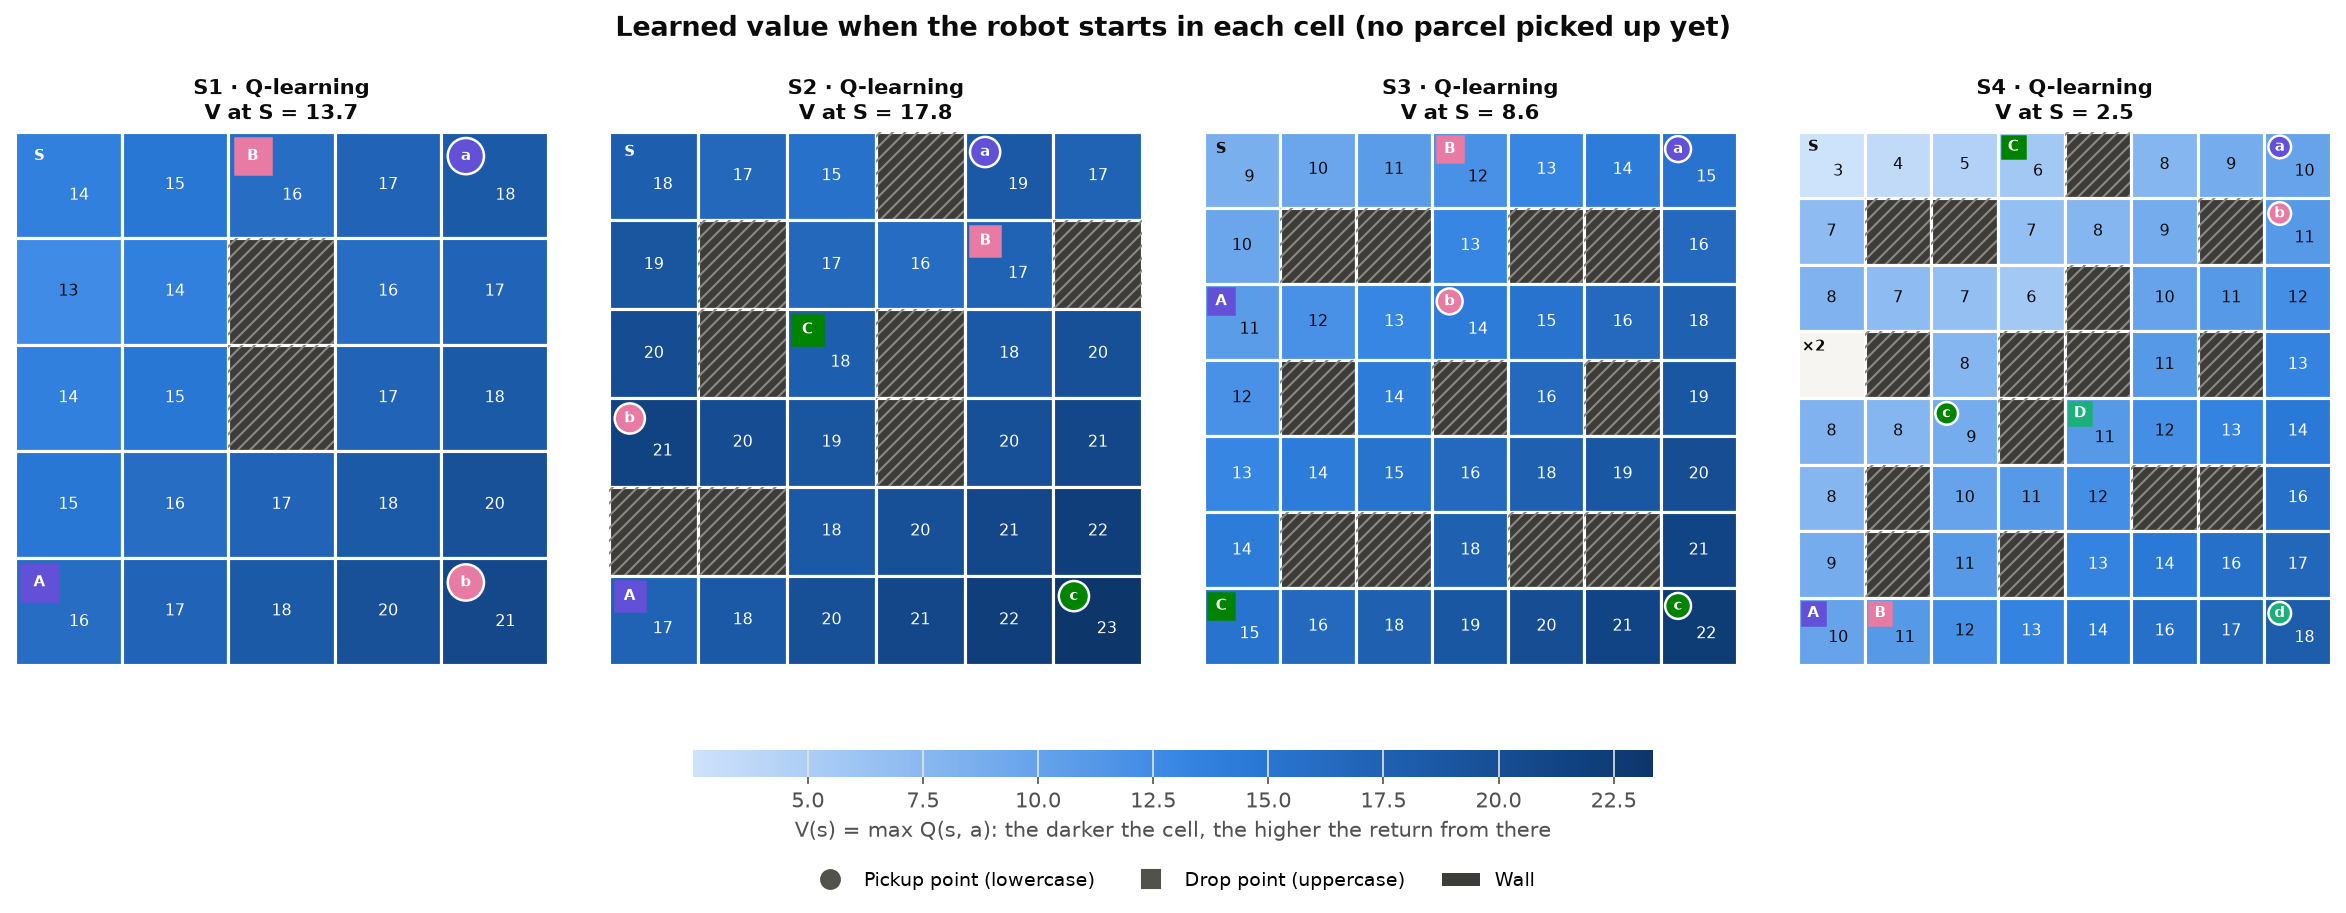
\includegraphics[width=\textwidth]{value_start.png}
\caption{Learned start value $V(s)=\max_a Q(s,a)$ in every cell of the four maps (Q-learning, no parcel picked up yet). Darker cells promise a higher return; hatched cells are walls.}
\label{fig:value_start}
\end{figure*}

\begin{figure}[!t]
\centering
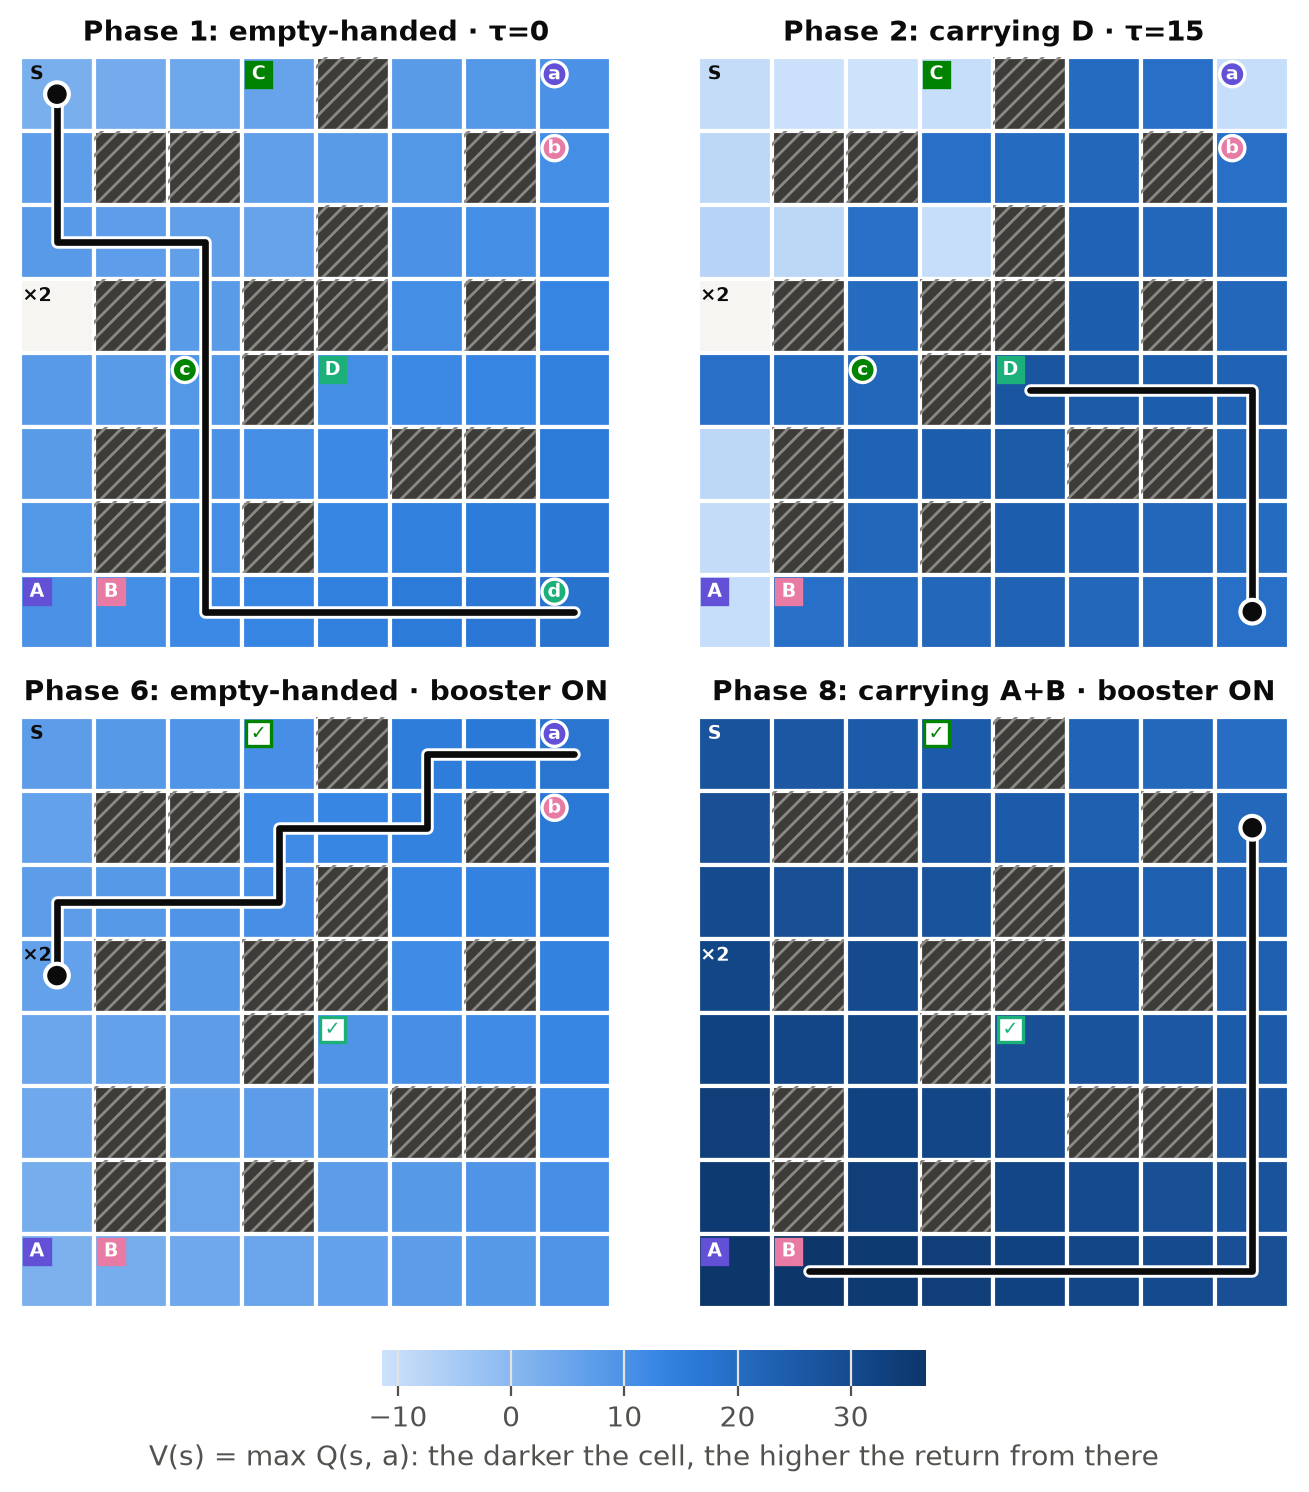
\includegraphics[width=\columnwidth]{value_S4_phases.png}
\caption{Learned value in four of the nine phases of the S4 route; the black line is the robot's route in that phase. In phase 2 the cells that can no longer meet D's deadline have negative values.}
\label{fig:value_phases}
\end{figure}

\subsection{Changing the Reward and the Environment}
Three variants were trained with Q-learning and 5 seeds (Table~\ref{tab:variants}, Fig.~\ref{fig:variants}). When the late penalty on S3 is removed, being late costs nothing, so the agent drops its priority for C and takes the 4-step-shorter order $B\rightarrow A\rightarrow C$. When the deadline is relaxed to 45 steps, delivering C last is still on time, so the agent also switches to $B\rightarrow A\rightarrow C$; the reachable states grow from 4,027 to 14,558, and all seeds remain optimal. Without the booster cell, S4 needs four separate trips ($D\rightarrow B\rightarrow C\rightarrow A$, 75 steps). In every case the learned policy matches the optimal solution in 5/5 seeds.

\begin{figure*}[!t]
\centering
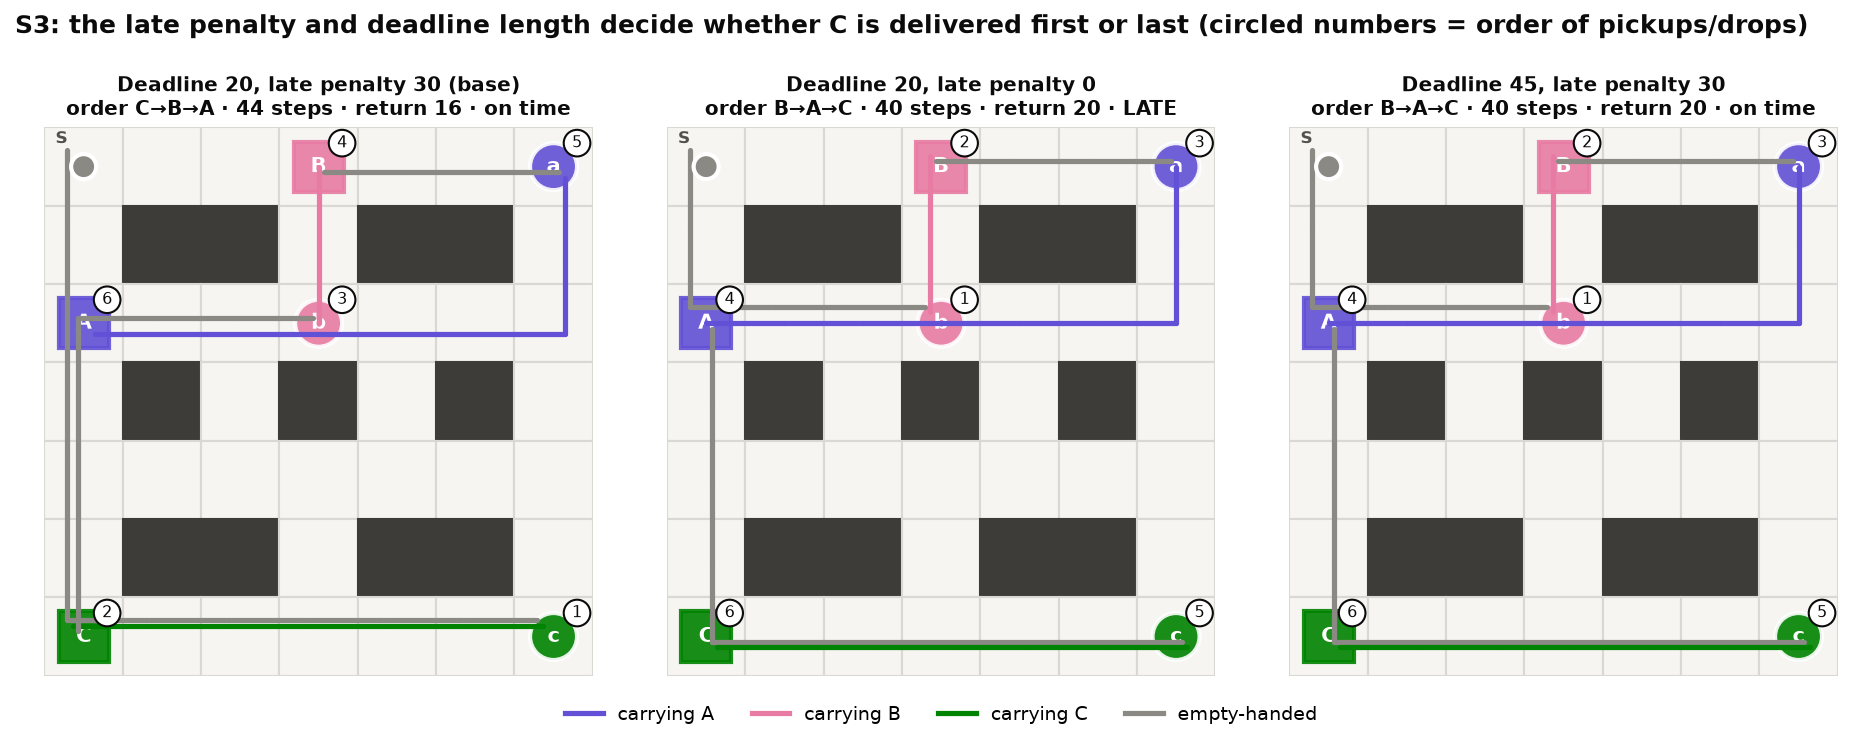
\includegraphics[width=0.8\textwidth]{reward_deadline.png}
\caption{S3 with three configurations. The base map delivers C first; with no late penalty or a 45-step deadline the order becomes $B\rightarrow A\rightarrow C$. Circled numbers give the order of pickup and drop events.}
\label{fig:variants}
\end{figure*}

\begin{table}[!t]
\caption{Reward and Environment Variants (Q-Learning, 5 Seeds)}
\label{tab:variants}
\centering
\footnotesize
\begin{adjustbox}{max width=\columnwidth}
\begin{tabular}{|p{2.5cm}|p{3.1cm}|p{1.4cm}|}
\hline
\textbf{Variant} & \textbf{Optimum (VI)} & \textbf{Learned} \\
\hline
S3 base: deadline 20, late penalty 30 & $C\rightarrow B\rightarrow A$, 44 steps, return 16 & optimal, on time \\
S3: late penalty 0 & $B\rightarrow A\rightarrow C$, 40 steps, return 20 (late) & optimal \\
S3: deadline 45 & $B\rightarrow A\rightarrow C$, 40 steps, return 20 (on time) & optimal \\
S4 base: booster cell & $D\rightarrow C\rightarrow B\rightarrow A$, 67 steps, return 13 & optimal \\
S4: no booster cell & $D\rightarrow B\rightarrow C\rightarrow A$, 75 steps, return 5 & optimal \\
\hline
\end{tabular}
\end{adjustbox}
\end{table}

\section{Discussion}
The results hold for a deterministic environment. There, Q-learning and MC ES benefit from noise-free targets; with stochastic moves (for example wheel slip) this advantage would shrink and the ranking could change. Exploring starts require a simulator that can place the robot in any state, which is easy here but not on a real robot. The deadline clock makes the state space grow linearly with the deadline length, and a Q table is tied to one grid, so every map is trained separately. Finally, the hyperparameters were tuned on the same four maps that are reported.

\section{Conclusion}
Tabular Q-learning, SARSA and MC ES all learn the optimal pickup and delivery order on four maps of increasing difficulty, reaching 100\% accuracy over every start cell in 5/5 seeds. Exploring starts and algorithm-specific exploration schedules are the decisive improvements, raising accuracy from 0--61\% to 100\% on the hardest maps. Q-learning learns fastest and most stably, MC ES is second, and SARSA needs about three times as many episodes. The learned policies react to changes in the late penalty, the deadline and the booster cell exactly as the optimal solution predicts, and the learned values make the deadline visible as a region of negative value. Future work includes a stochastic version of the environment, Expected SARSA and Q($\lambda$), and function approximation so that one model can serve several maps.

\begin{thebibliography}{00}
\bibitem{b9} S. N. Parragh, K. F. Doerner, and R. F. Hartl, ``A survey on pickup and delivery problems. Part II: Transportation between pickup and delivery locations,'' \textit{J. f\"{u}r Betriebswirtschaft}, vol. 58, no. 2, pp. 81--117, 2008.
\bibitem{b4} T. G. Dietterich, ``Hierarchical reinforcement learning with the MAXQ value function decomposition,'' \textit{J. Artif. Intell. Res.}, vol. 13, pp. 227--303, 2000.
\bibitem{b5} M. Towers \textit{et al.}, ``Gymnasium: A standard interface for reinforcement learning environments,'' arXiv:2407.17032, 2024.
\bibitem{b2} C. J. C. H. Watkins and P. Dayan, ``Q-learning,'' \textit{Machine Learning}, vol. 8, no. 3--4, pp. 279--292, 1992.
\bibitem{b3} G. A. Rummery and M. Niranjan, ``On-line Q-learning using connectionist systems,'' Cambridge Univ. Eng. Dept., Tech. Rep. CUED/F-INFENG/TR 166, 1994.
\bibitem{b1} R. S. Sutton and A. G. Barto, \textit{Reinforcement Learning: An Introduction}, 2nd ed. Cambridge, MA, USA: MIT Press, 2018.
\bibitem{b7} S. Singh, T. Jaakkola, M. L. Littman, and C. Szepesv\'{a}ri, ``Convergence results for single-step on-policy reinforcement-learning algorithms,'' \textit{Machine Learning}, vol. 38, no. 3, pp. 287--308, 2000.
\bibitem{b8} R. Bellman, \textit{Dynamic Programming}. Princeton, NJ, USA: Princeton Univ. Press, 1957.
\bibitem{b6} S. K. Lam, A. Pitrou, and S. Seibert, ``Numba: A LLVM-based Python JIT compiler,'' in \textit{Proc. 2nd Workshop LLVM Compiler Infrastructure in HPC}, 2015, pp. 1--6.
\end{thebibliography}

\end{document}
